\fancyhead{}
\fancyfoot{}
\cfoot{\thepage}

\lhead{Resultados}

\chapter{Resultados}

Para garantizar resultados precisos durante la evaluación del sistema de asistencia basado en reconocimiento facial, se definió un entorno de pruebas controlado. A continuación, se detallan las características del hardware y software utilizados, así como la versión del sistema y los módulos activados durante las pruebas.

\section{Figuras y Tablas}

\begin{table}[H]
    \centering
    \caption{Componentes de hardware y software utilizados en el sistema. [Figura Propia]}
    \label{tab:entorno_pruebas}
    \renewcommand{\arraystretch}{1.3}
    \begin{tabular}{|p{5cm}|p{9cm}|}
        \hline
        \textbf{Elemento} & \textbf{Descripción} \\ \hline

        Modelo de cámara & Cámara web HD 720p \\ \hline

        Servidor & AMD Ryzen 7 7735HS, 16 GB RAM, SSD 512 GB, Windows 11 Home \\ \hline

        Lenguaje de programación & Python 3.12.11 \\ \hline

        Framework backend & Flask \\ \hline

        Base de datos & PostgreSQL 18 \\ \hline

        Framework frontend & React, Bootstrap \\ \hline

        Librerías & OpenCV, NumPy, Pandas, Ultralytics, DeepFace, TensorFlow-CPU==2.13.0, SQLAlchemy, Flask-CORS, Flask-JWT-Extended, Omegaconf, Matplotlib, Pillow \\ \hline

        Versión del sistema desarrollado & v1.0 Beta \\ \hline

        Módulos activados & Captura de imagen, Preprocesamiento, Detección facial, Reconocimiento, Registro en base de datos, Reporte de asistencia \\ \hline
    \end{tabular}
\end{table}



\subsection{Errores detectados y ajustes aplicados}

Durante la etapa de pruebas, se identificaron ciertos errores recurrentes en el funcionamiento del sistema, principalmente relacionados con la precisión del reconocimiento facial. A continuación, se presenta una tabla con los tipos de errores detectados, su causa y las acciones de mitigación implementadas para mejorar el desempeño.

\begin{table}[H]
    \centering
    \caption{Errores frecuentes y acciones de mitigación. [Figura Propia]}
    \label{tab:errores_ajustes}
    \renewcommand{\arraystretch}{1.3}
    \begin{tabular}{|p{4cm}|p{6cm}|p{4.5cm}|}
        \hline
        \textbf{Tipo de error} & \textbf{Causa identificada} & \textbf{Ajuste o solución aplicada} \\ \hline

        Falsos positivos & Umbral de similitud fijo no adecuado a la variación entre usuarios & Umbral ajustado dinámicamente según el número y diversidad de imágenes por usuario \\ \hline

        Reconocimiento inexacto con poca luz & Capturas en entornos con baja iluminación o sombras & Aplicación de mejora de contraste y normalización de imagen \\ \hline

        Procesamiento lento & Comparación directa con todos los embeddings registrados & Filtrado previo por clase y reducción del número de comparaciones simultáneas \\ \hline
    \end{tabular}
\end{table}

\begin{table}[H]
\centering
\caption{Configuración de umbral centrada en 0.45 y resultado esperado. [Figura Propia]}
\label{tab:umbral_045}
\renewcommand{\arraystretch}{1.3}
\begin{tabular}{|c|p{5cm}|p{5.8cm}|}
\hline
\textbf{Umbral ($\texttt{min\_dist} >$ ?)} & \textbf{Resultado esperado} & \textbf{Notas} \\ \hline

$> 0.25$ & Reconocimiento muy estricto & Alta precisión, pero puede fallar con cambios leves de luz o expresión. \\ \hline

$> 0.35$ & Recomendado en entornos controlados & Mantiene un equilibrio adecuado entre precisión y estabilidad. \\ \hline

$> 0.45$ & Valor equilibrado & Buen compromiso entre exactitud y tolerancia, utilizado como referencia base del sistema. \\ \hline

$> 0.60$ & Reconocimiento flexible & Acepta pequeñas variaciones de ángulo o iluminación sin perder confiabilidad. \\ \hline

$> 0.75$ & Reconocimiento permisivo & Mayor tolerancia, con posibilidad de falsos positivos en rostros similares. \\ \hline
\end{tabular}
\end{table}



\subsection{Configuraciones y resultados obtenidos}

\textbf{Configuración 1: Umbral 0.25}

\begin{figure}[H]
    \centering
    
\includegraphics[width=0.9\textwidth]{capitulo_05/imagenes/1.jpg}
    \caption{Fragmento de código utilizado para configurar el umbral de reconocimiento.[Figura Propia]}
\end{figure}

\begin{figure}[H]
    \centering
    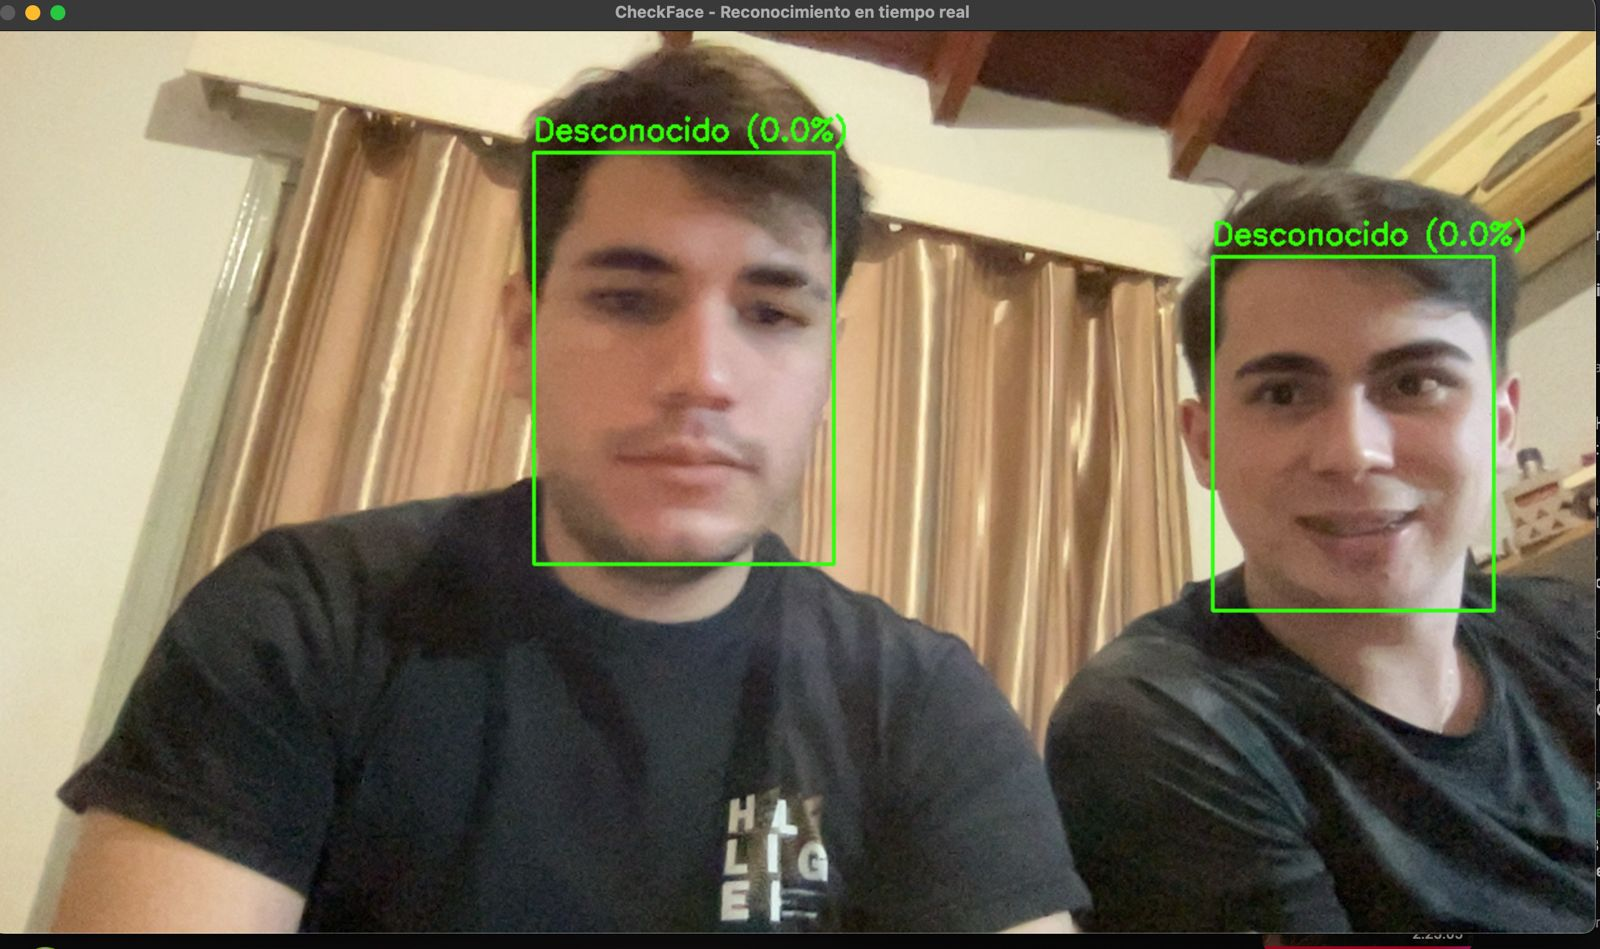
\includegraphics[width=0.7\textwidth]{capitulo_05/imagenes/umbral_1.0_30.jpg}
    \caption{Muy estricto, reconoce solo rostros casi idénticos.[Figura Propia]}
\end{figure}

\newpage

\textbf{Configuración 2: Umbral 0.35}

\begin{figure}[H]
    \centering
    
\includegraphics[width=0.9\textwidth]{capitulo_05/imagenes/2.png}
    \caption{Fragmento de código utilizado para configurar el umbral de reconocimiento.[Figura Propia]}
\end{figure}

\begin{figure}[H]
    \centering
    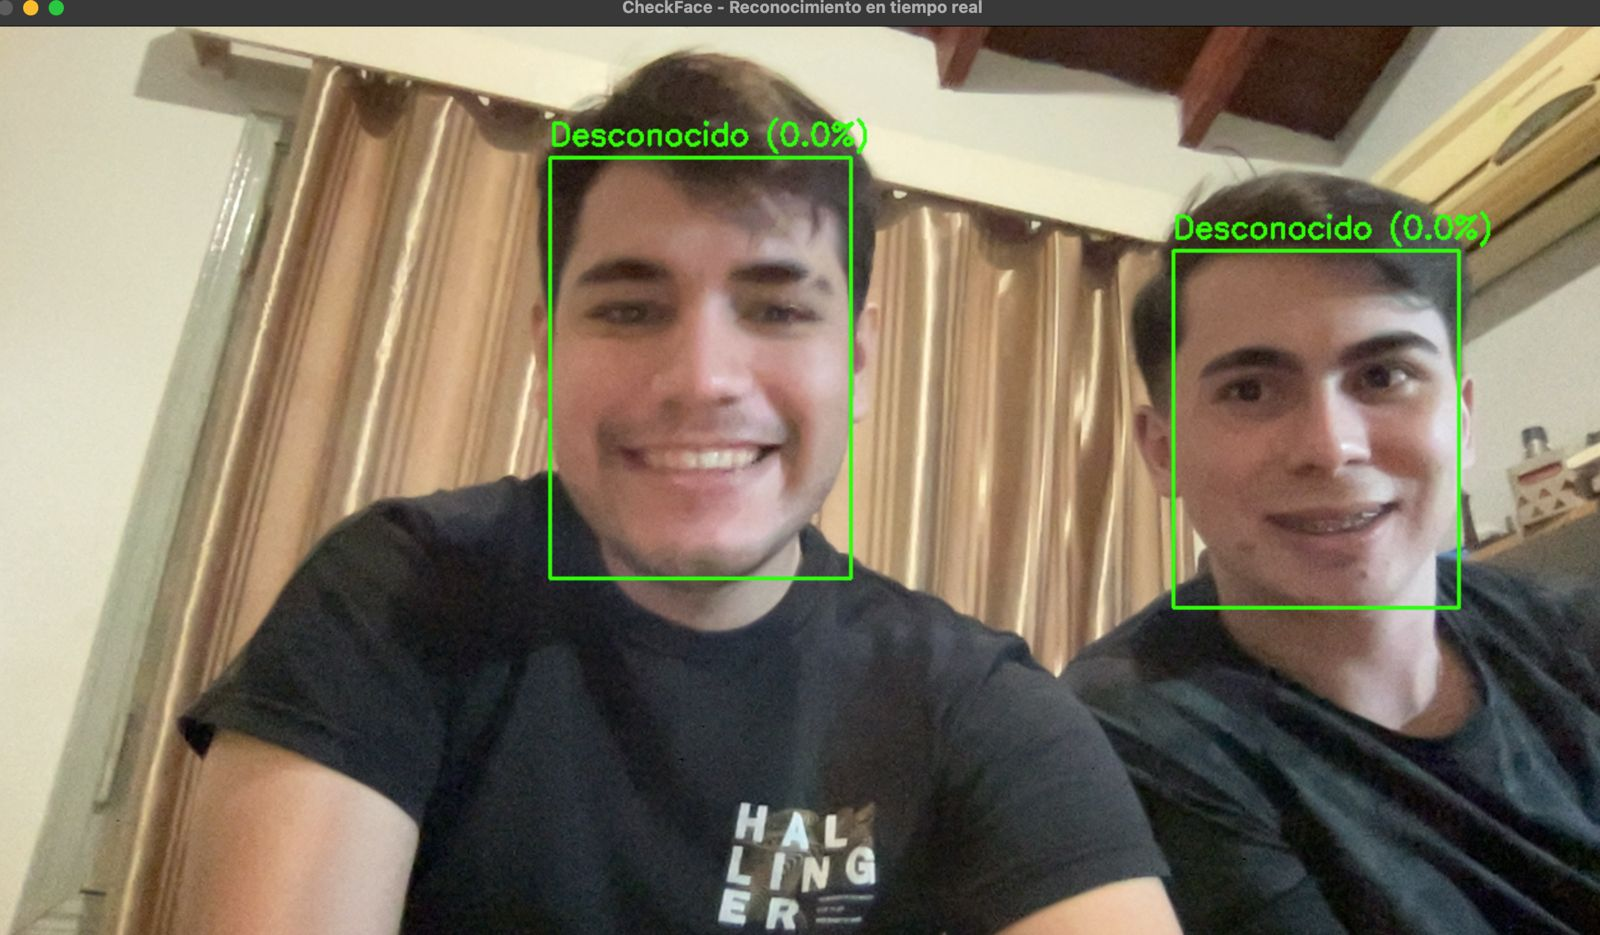
\includegraphics[width=0.85\textwidth]{capitulo_05/imagenes/1.3_min_dist25.jpg}
    \caption{Estricto, buena precisión, pero sensible a luz o expresión.[Figura Propia]}
\end{figure}

\newpage

\textbf{Configuración 3: Umbral 0.45}

\begin{figure}[H]
    \centering
    
\includegraphics[width=0.85\textwidth]{capitulo_05/imagenes/3.png}
    \caption{Fragmento de código utilizado para configurar el umbral de reconocimiento.[Figura Propia]}
\end{figure}

\begin{figure}[H]
    \centering
    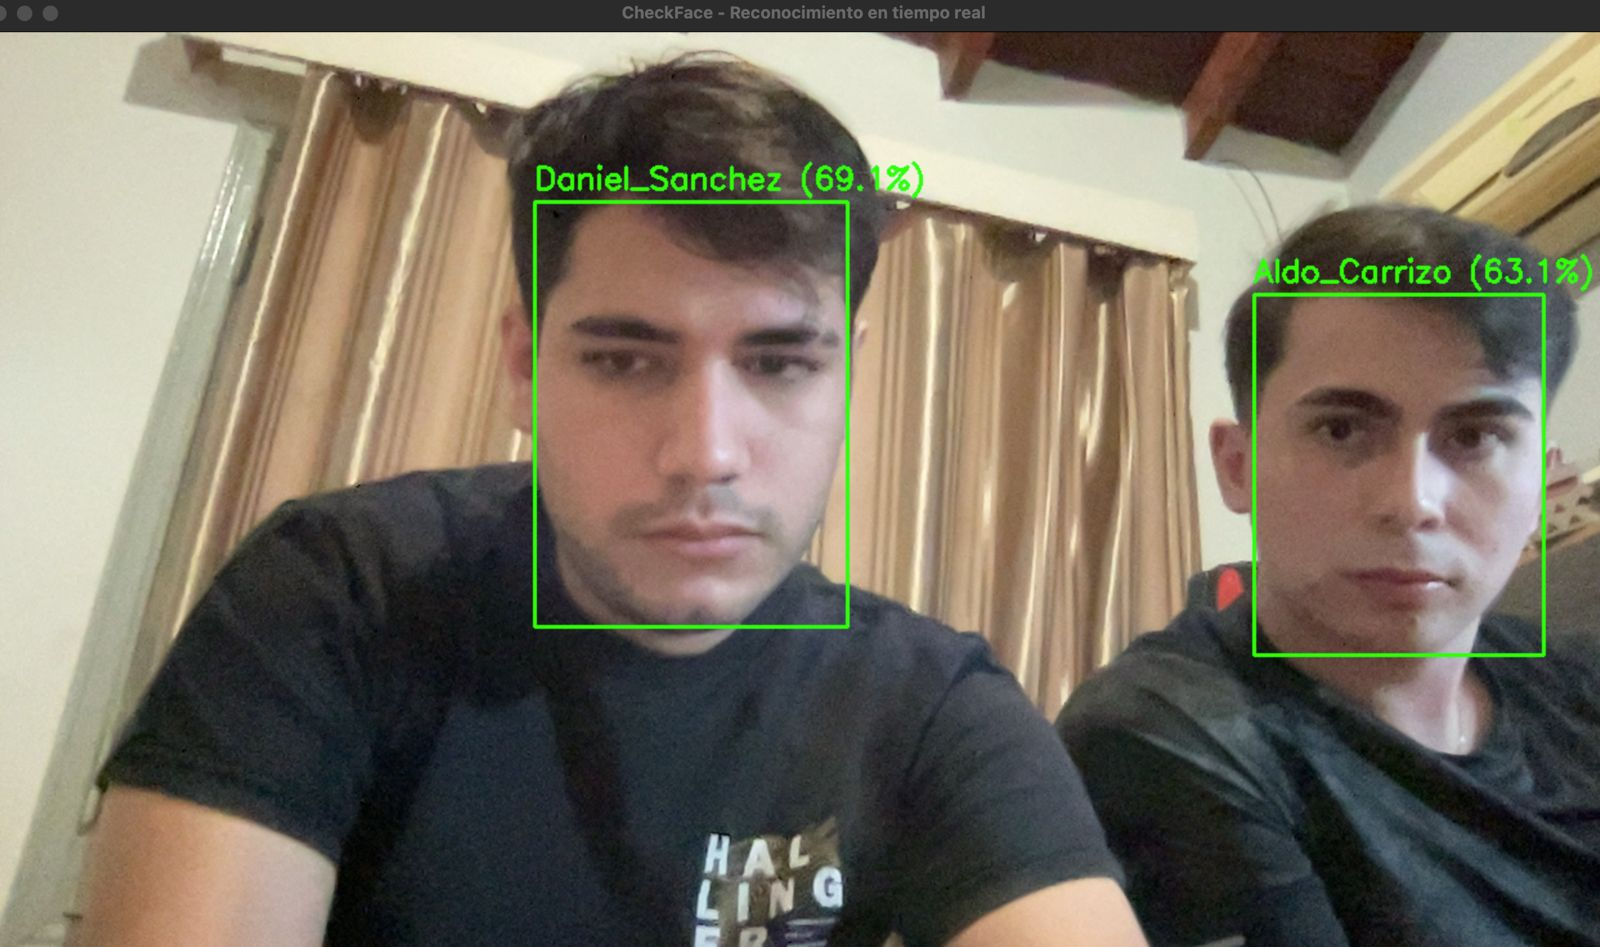
\includegraphics[width=0.8\textwidth]{capitulo_05/imagenes/6.6.jpg}
    \caption{Equilibrado, balance entre precisión y tolerancia.[Figura Propia]}
\end{figure}

\newpage


\textbf{Configuración 4: Umbral 0.60}

\begin{figure}[H]
    \centering
    
\includegraphics[width=0.8\textwidth]{capitulo_05/imagenes/4.png}
    \caption{Fragmento de código utilizado para configurar el umbral de reconocimiento.[Figura Propia]}
\end{figure}

\begin{figure}[H]
    \centering
    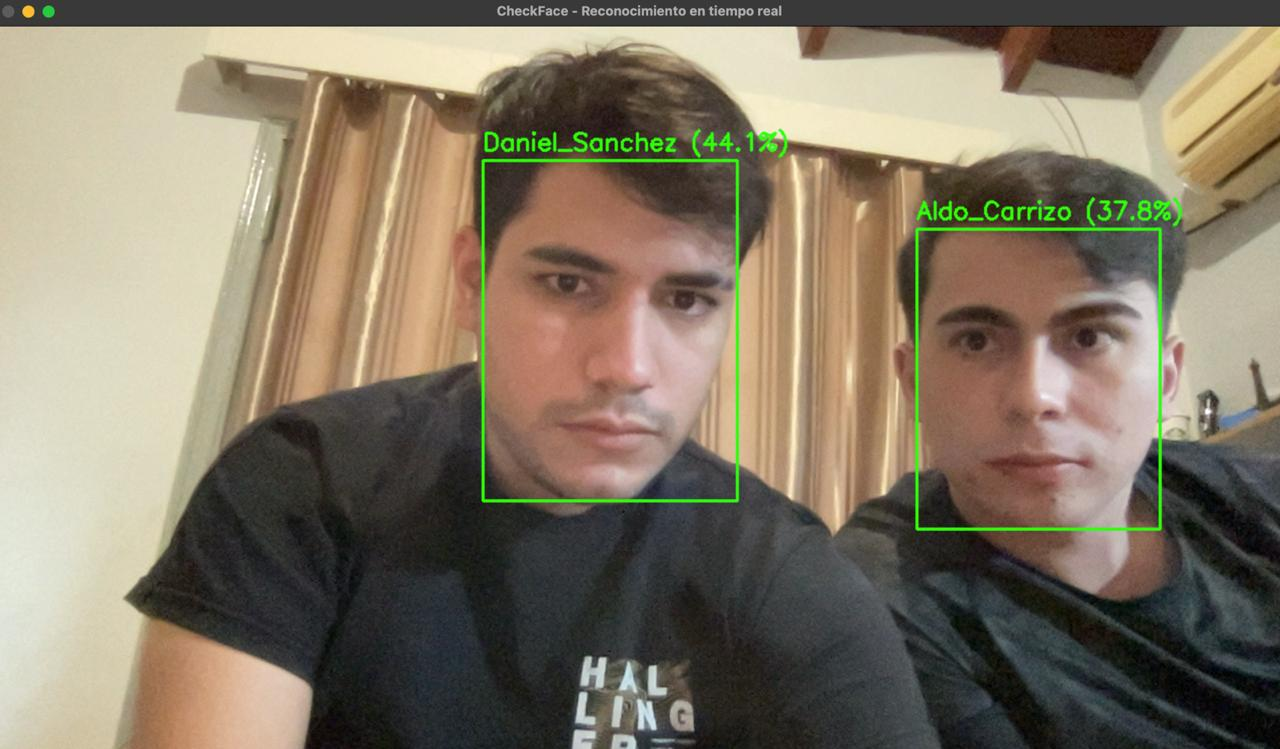
\includegraphics[width=0.8\textwidth]{capitulo_05/imagenes/4.4.jpg}
    \caption{Moderadamente flexible, admite pequeñas variaciones.[Figura Propia]}
\end{figure}


\newpage


\textbf{Configuración 5: 0.75}

\begin{figure}[H]
    \centering
    
\includegraphics[width=0.8\textwidth]{capitulo_05/imagenes/5.png}
    \caption{Fragmento de código utilizado para configurar el umbral de reconocimiento.[Figura Propia]}
\end{figure}

\begin{figure}[H]
    \centering
    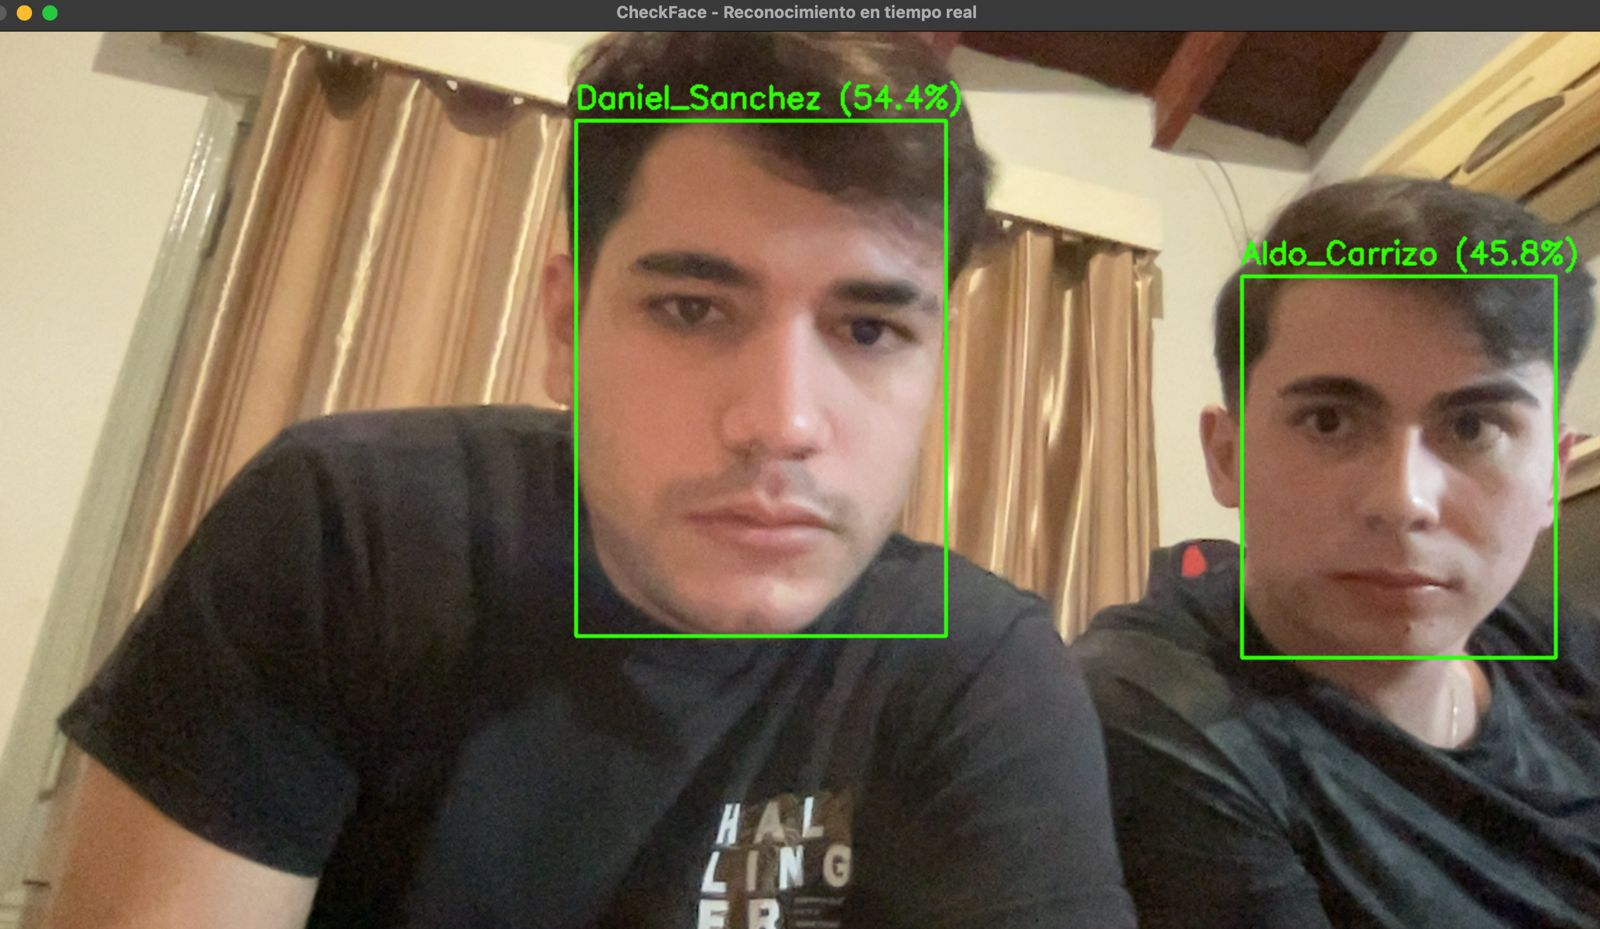
\includegraphics[width=0.8\textwidth]{capitulo_05/imagenes/5.5.jpg}
    \caption{Puede aceptar coincidencias con diferencias notables.[Figura Propia]}
\end{figure}


\newpage


\section{Resultados finales del sistema en condiciones reales de un aula}


\textbf{Configuración 1: Prueba inicial con iluminación máxima}

Se presenta una de las primeras pruebas realizadas en el aula, bajo iluminación artificial máxima. En la escena participaron cuatro personas, dos registradas y dos no registradas en el sistema. El modelo reconoció correctamente a las registradas, asignando niveles de similitud superiores al 80\,\%, mientras que las demás fueron clasificadas como “Desconocido (0.0\,\%)”, demostrando su capacidad para diferenciar usuarios registrados en condiciones óptimas de luz.

\begin{figure}[H]
    \centering
    
\includegraphics[width=1\textwidth]{capitulo_05/resultados_aula/1.jpg}
    \caption{Prueba inicial del sistema bajo condiciones de iluminación máxima, con detección de personas registradas y no registradas. [Figura Propia]}
    \label{fig:prueba1}
\end{figure}

\textbf{Configuración 2: Evaluación de estabilidad con iluminación uniforme}

Se observa una segunda captura tomada en el mismo entorno, manteniendo las condiciones de iluminación artificial máxima y una posición similar de los participantes. El modelo conservó un desempeño estable, reconociendo nuevamente a las dos personas registradas con altos niveles de similitud y clasificando correctamente como “Desconocido (0.0\,\%)” a quienes no estaban en la base de datos. Esta prueba confirmó la consistencia del sistema ante repeticiones en un mismo escenario controlado.

\begin{figure}[H]
    \centering
    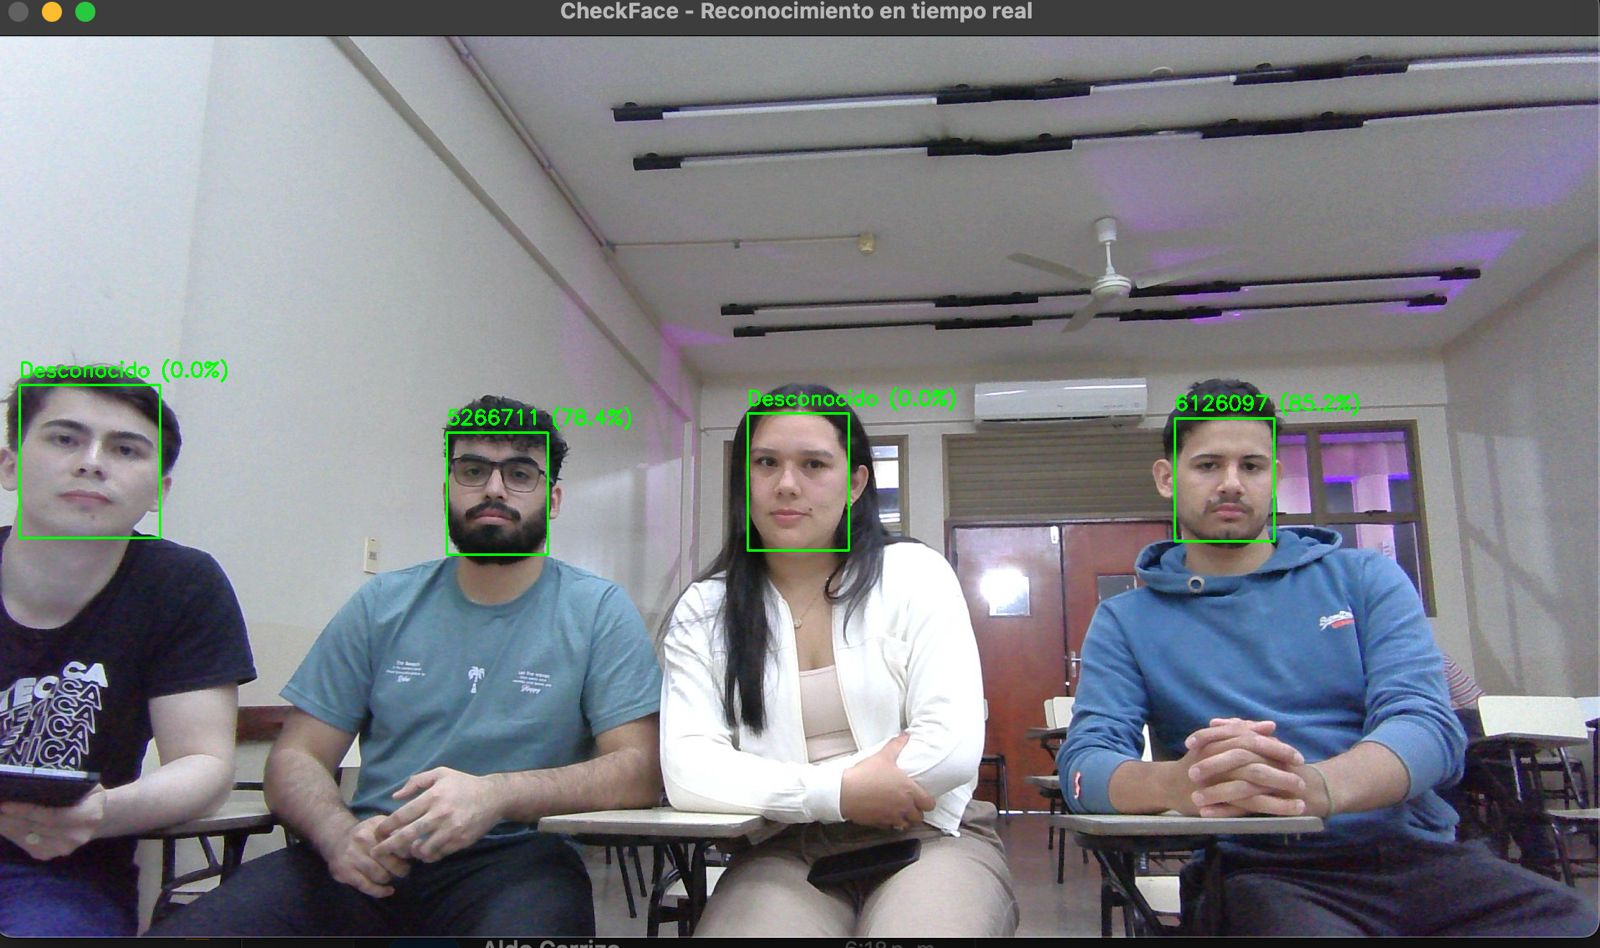
\includegraphics[width=1\textwidth]{capitulo_05/resultados_aula/2.jpg}
    \caption{Segunda prueba con iluminación uniforme, evidenciando estabilidad en las detecciones. [Figura Propia]}
    \label{fig:prueba2}
\end{figure}

\textbf{Configuración 3: Reconocimiento con variación leve de postura y uso de accesorios}

En la Figura~\ref{fig:prueba3} se presenta una prueba en la que los participantes modificaron levemente su postura y expresión facial respecto a las capturas anteriores. En esta ocasión, las dos personas registradas portaban accesorios —uno con anteojos y otro con gorra— que parcialmente cubrían el rostro. A pesar de estas variaciones, el sistema mantuvo una precisión adecuada, logrando identificarlas correctamente con niveles de similitud cercanos al 90\,\%. Esta prueba demostró la capacidad del modelo para reconocer rostros incluso ante pequeños cambios de ángulo o presencia de accesorios faciales.

\begin{figure}[H]
    \centering
    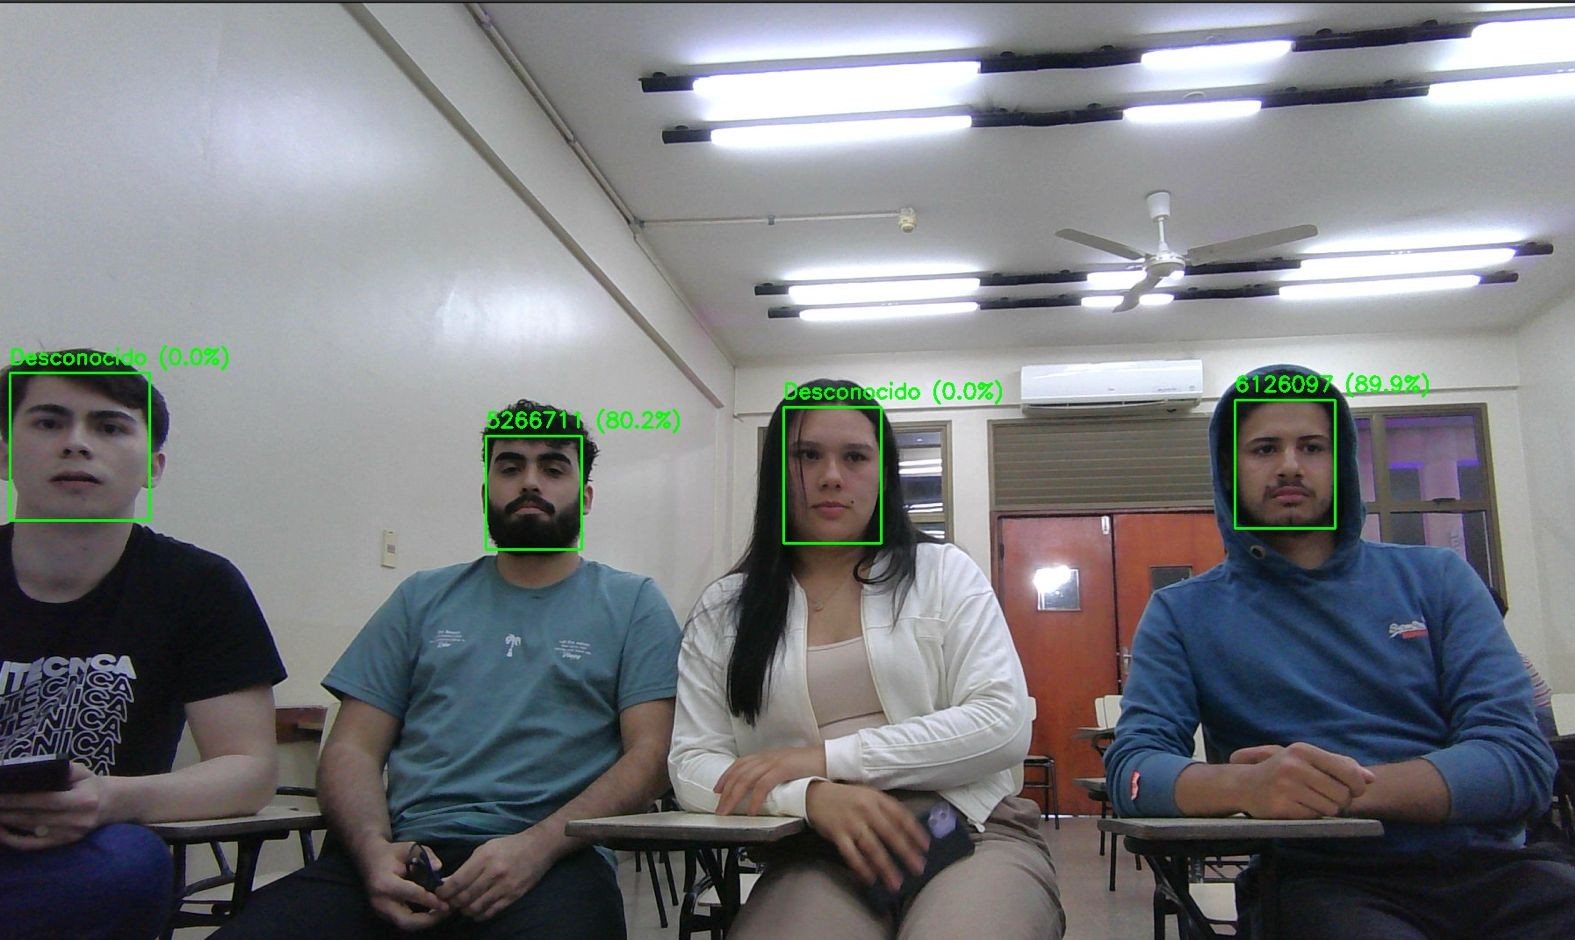
\includegraphics[width=1\textwidth]{capitulo_05/resultados_aula/4.jpg}
    \caption{Prueba con variaciones leves de postura y uso de accesorios, manteniendo altos niveles de reconocimiento. [Figura Propia]}
    \label{fig:prueba3}
\end{figure}

\textbf{Configuración 4: Evaluación a mayor distancia}

En la Figura~\ref{fig:prueba4} se presenta una prueba en la que la cámara fue ubicada a una distancia superior a los cinco metros de los participantes. Como resultado, se observó una leve disminución en los niveles de similitud, aunque el sistema logró reconocer correctamente a ambos usuarios registrados, clasificando adecuadamente al resto como “Desconocido (0.0\,\%)”. Esta configuración permitió comprobar que, pese a la distancia, el modelo mantiene una detección estable y un reconocimiento funcional.

\begin{figure}[H]
    \centering
    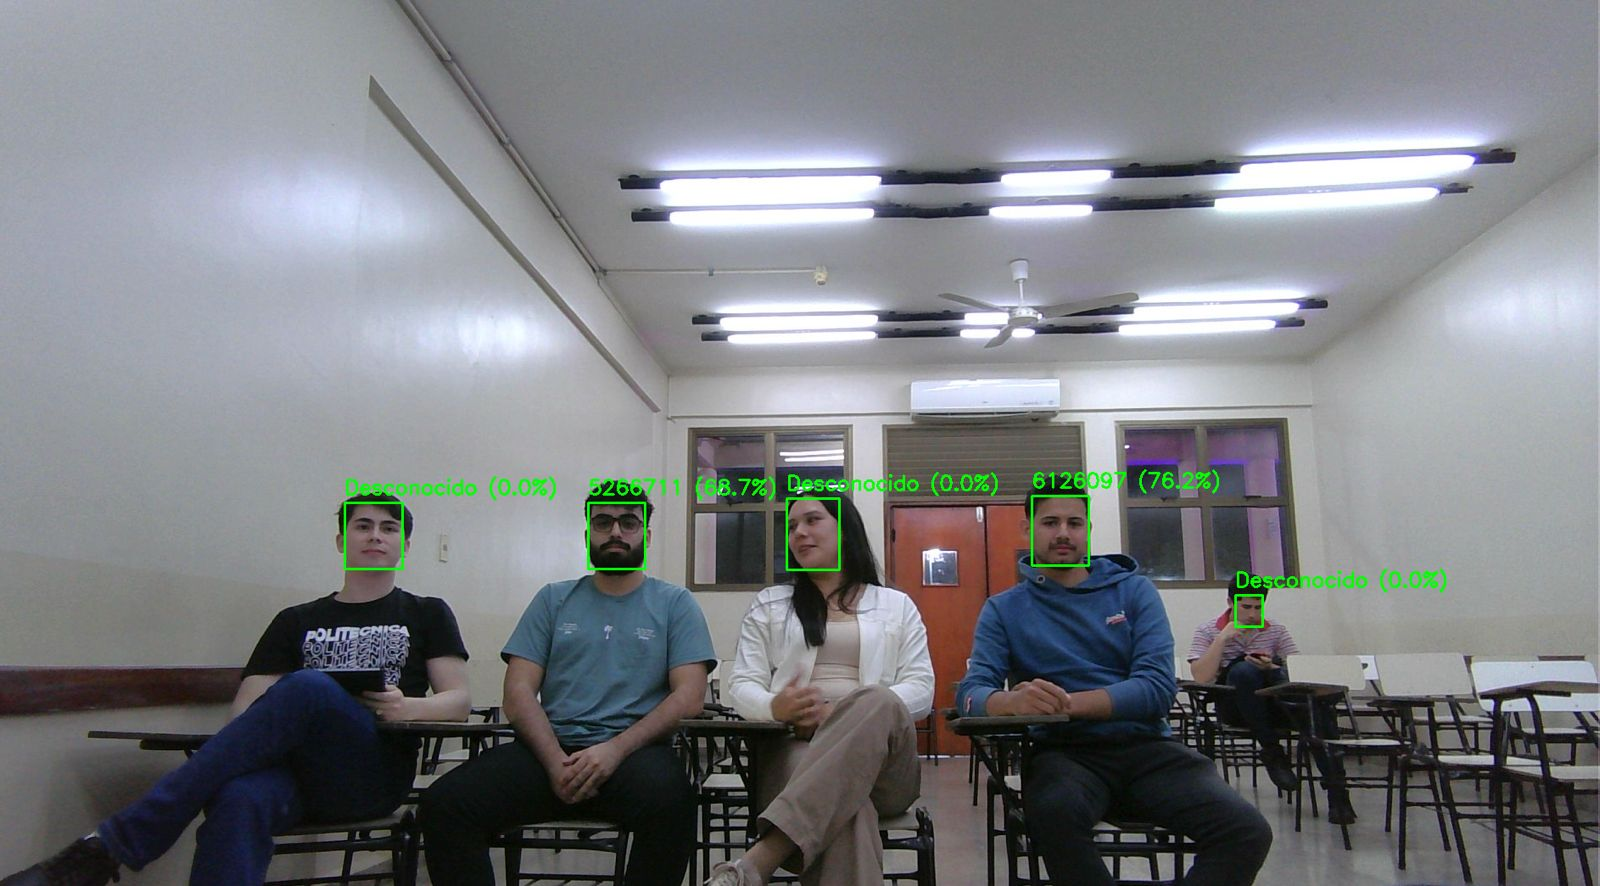
\includegraphics[width=1\textwidth]{capitulo_05/resultados_aula/5.jpg}
    \caption{Prueba a mayor distancia, con leve disminución en la similitud pero reconocimiento correcto de los usuarios registrados. [Figura Propia]}
    \label{fig:prueba4}
\end{figure}




\textbf{Configuración 5: Evaluación con iluminación reducida}

En la Figura~\ref{fig:prueba5} se muestra una prueba realizada con una iluminación inferior al 50\,\% de la capacidad total de la sala. Esta condición permitió analizar el impacto de la luz sobre la precisión del sistema. Se observó una disminución natural en los niveles de similitud, aunque el modelo mantuvo la detección de todos los rostros y logró reconocer correctamente a los usuarios registrados. Los resultados evidencian la influencia directa de la iluminación ambiental en el rendimiento del reconocimiento facial.

\begin{figure}[H]
    \centering
    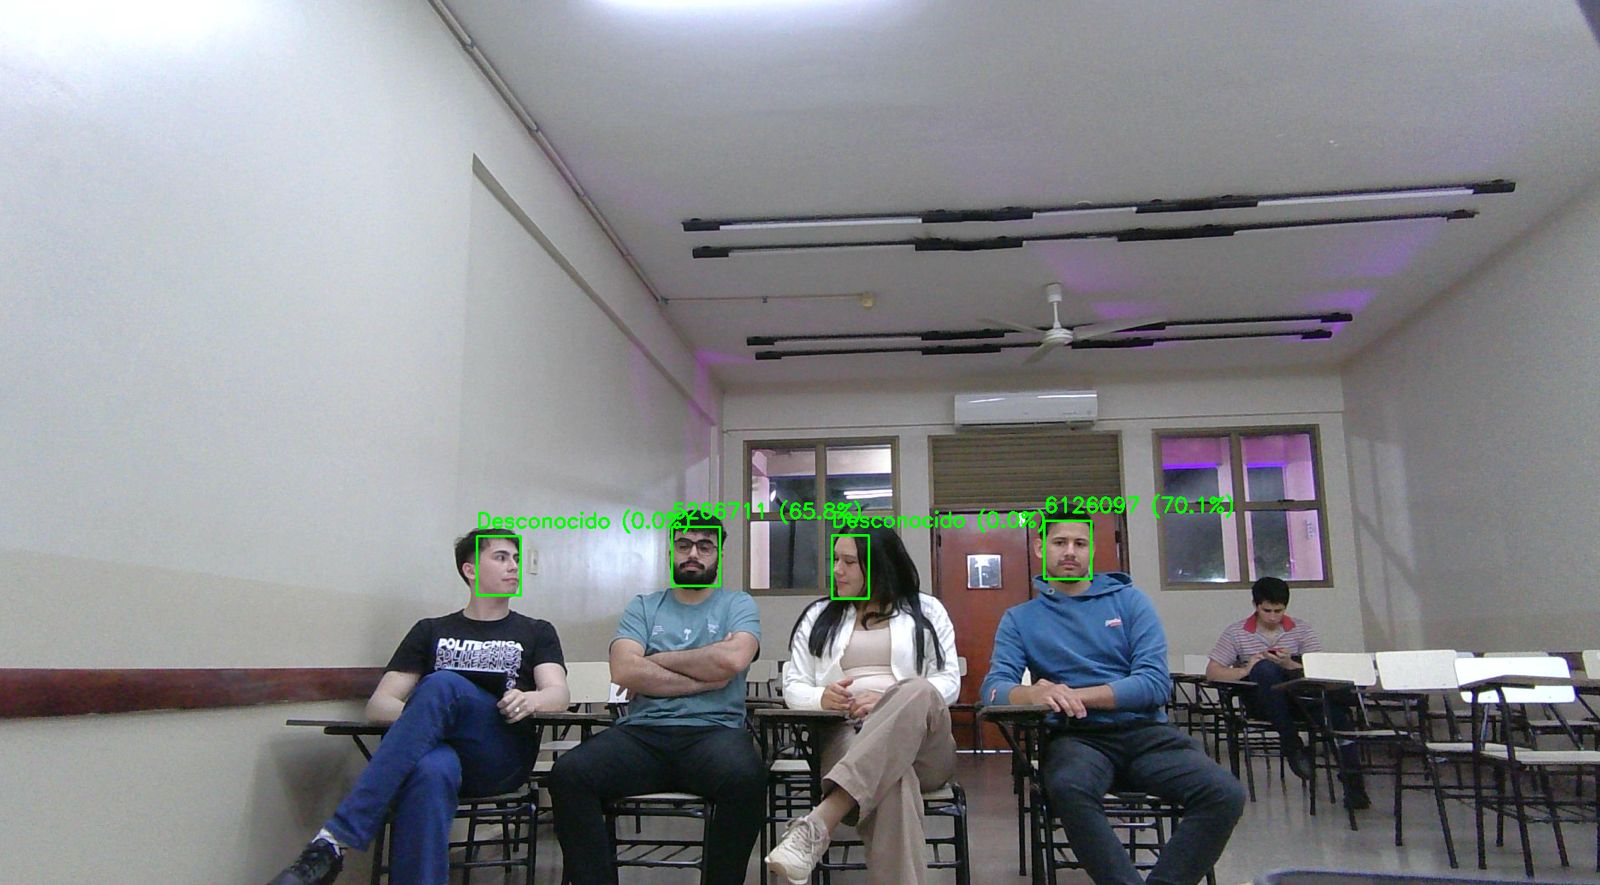
\includegraphics[width=1\textwidth]{capitulo_05/resultados_aula/6.jpg}
    \caption{Prueba con iluminación reducida, mostrando una disminución natural en la precisión de reconocimiento. [Figura Propia]}
    \label{fig:prueba5}
\end{figure}


\textbf{Configuración 6: Prueba con iluminación mínima}

En la Figura~\ref{fig:prueba6} se presenta la prueba realizada bajo las condiciones de iluminación más bajas posibles dentro del aula. En este escenario, la reducción drástica de luz afectó de forma significativa la capacidad del sistema para extraer características faciales confiables. Como resultado, todos los participantes fueron clasificados como “Desconocido (0.0\,\%)”, evidenciando la dependencia del modelo respecto a una iluminación adecuada para lograr un reconocimiento efectivo.

\begin{figure}[H]
    \centering
    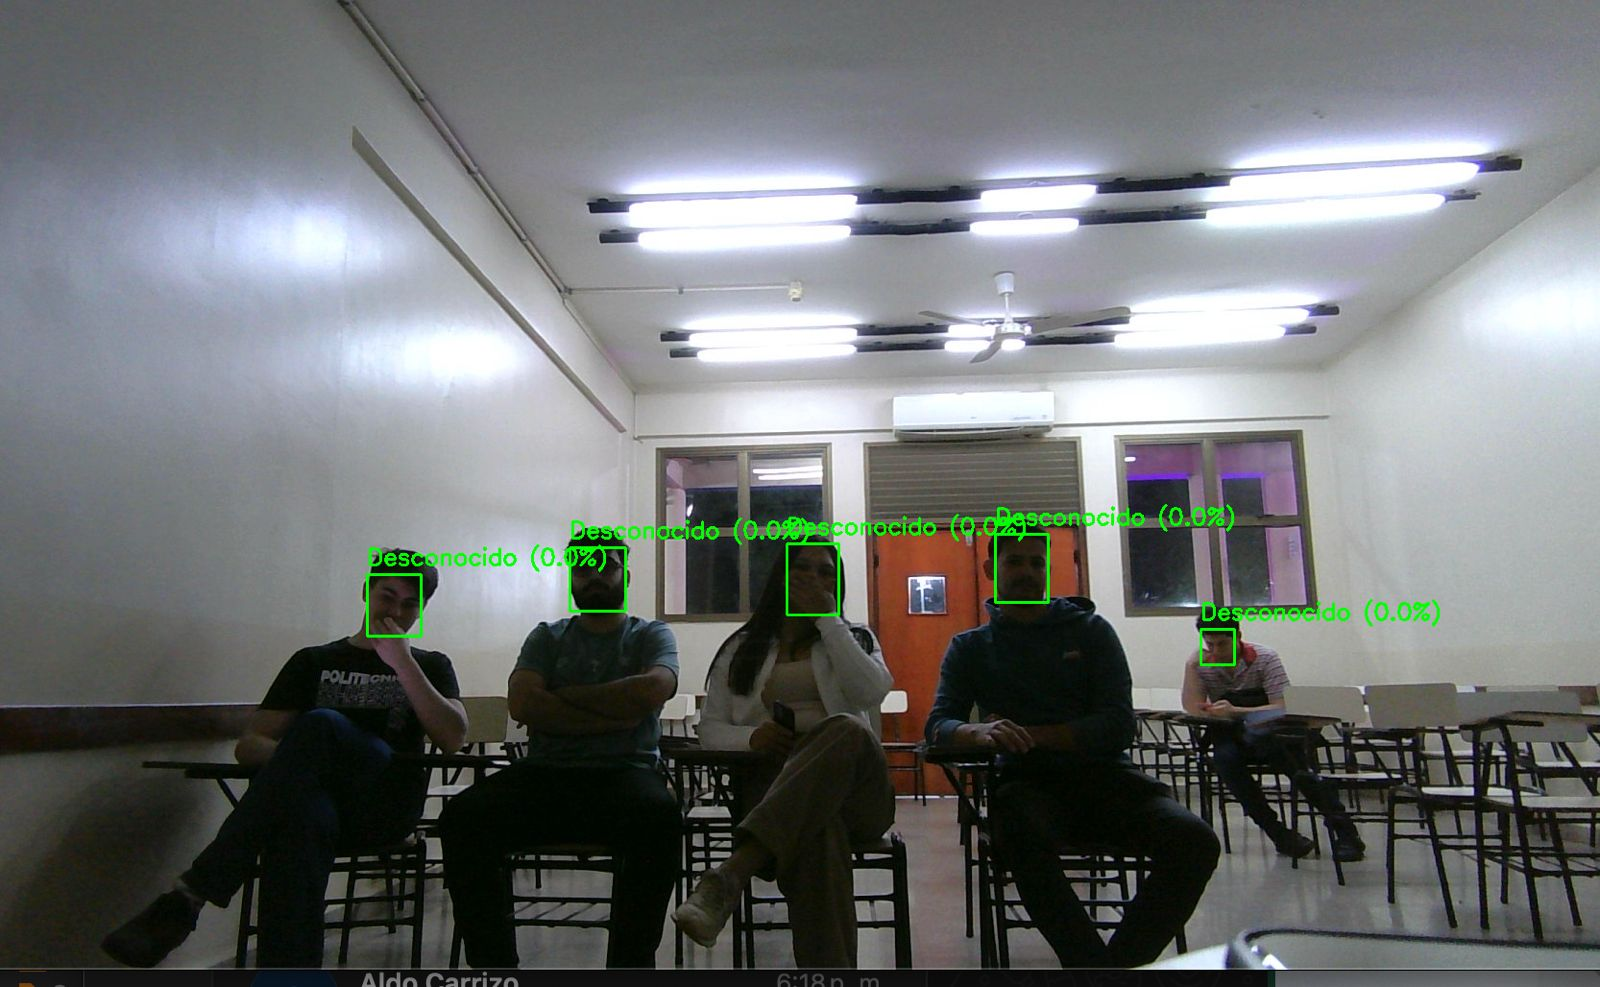
\includegraphics[width=1\textwidth]{capitulo_05/resultados_aula/7.jpg}
    \caption{Prueba con iluminación mínima, donde el sistema no logró reconocer a los participantes. [Figura Propia]}
    \label{fig:prueba6}
\end{figure}

\textbf{Configuración 7: Cambio de posición de los participantes registrados}

En la Figura~\ref{fig:prueba7} se muestra una prueba realizada bajo condiciones normales de iluminación, donde se modificó únicamente la posición de los participantes registrados dentro del aula. A pesar del cambio en la ubicación y el ángulo de los rostros, el sistema logró reconocer correctamente a los usuarios registrados con niveles de similitud superiores al 70\,\%. Esta prueba confirmó la capacidad del modelo para mantener la identificación aun cuando varía la posición espacial de los sujetos dentro del encuadre.

\begin{figure}[H]
    \centering
    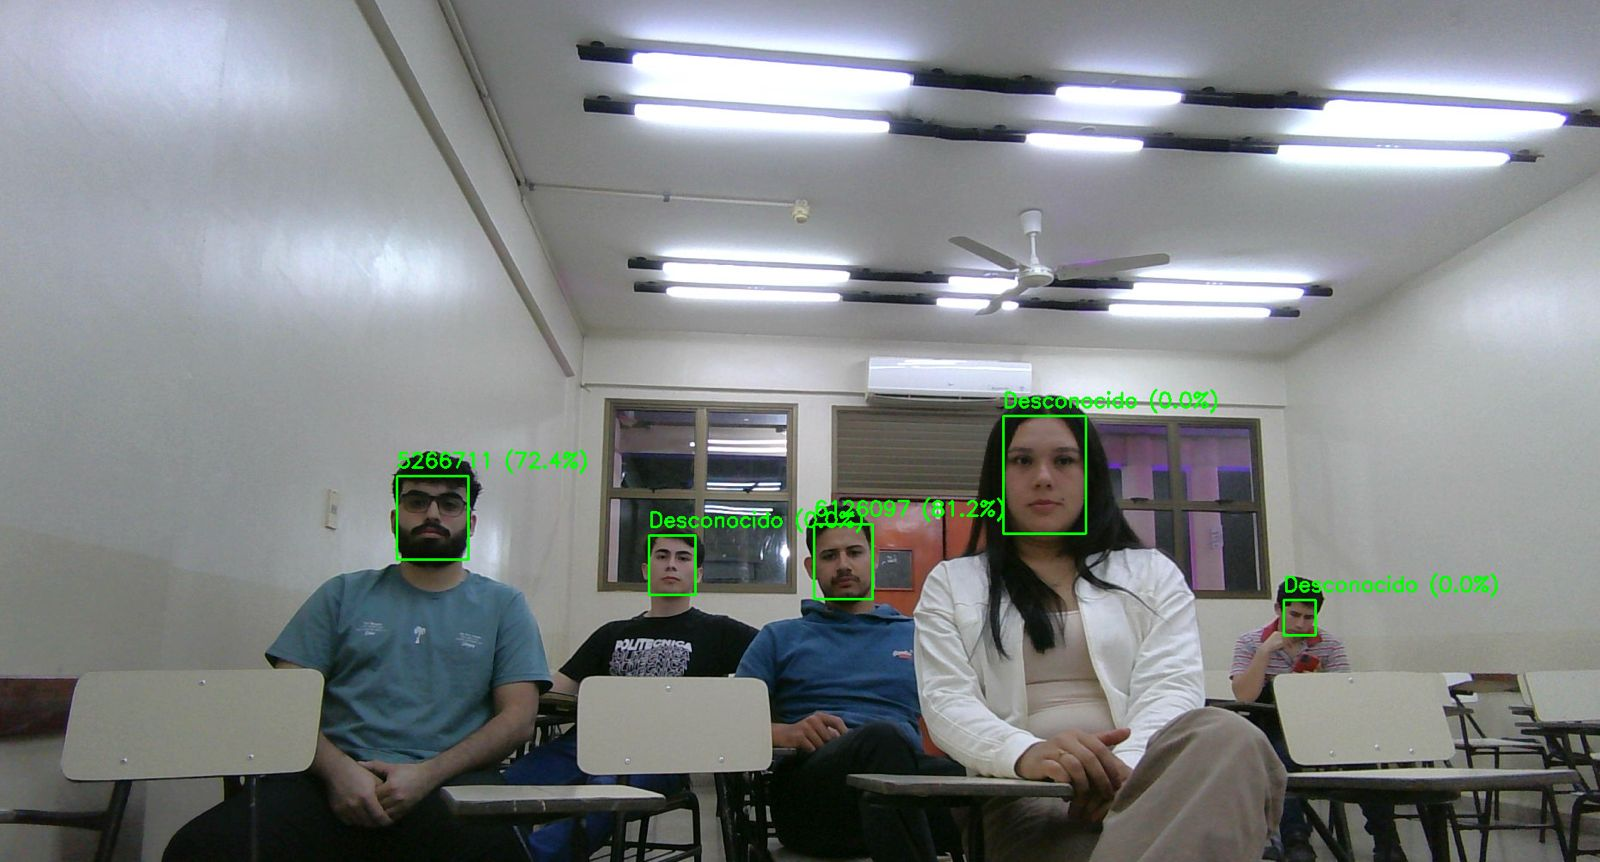
\includegraphics[width=1\textwidth]{capitulo_05/resultados_aula/10.jpg}
    \caption{Prueba con condiciones normales de iluminación y cambio de posición de los participantes registrados. [Figura Propia]}
    \label{fig:prueba7}
\end{figure}


\textbf{Configuración 8: Prueba con variación en la altura de la cámara}

En la Figura~\ref{fig:prueba8} se muestra una prueba realizada bajo condiciones normales de iluminación, pero con una variación significativa en la posición de la cámara. A diferencia de las pruebas anteriores —donde la cámara se ubicó a la altura de la mesa del profesor—, en esta ocasión se colocó a una altura aproximada de 2,30 metros. A pesar del ángulo descendente, el sistema mantuvo un reconocimiento estable de los participantes registrados, con niveles de similitud superiores al 70\,\%. Esta configuración permitió comprobar la adaptabilidad del modelo ante cambios de perspectiva vertical.

\begin{figure}[H]
    \centering
    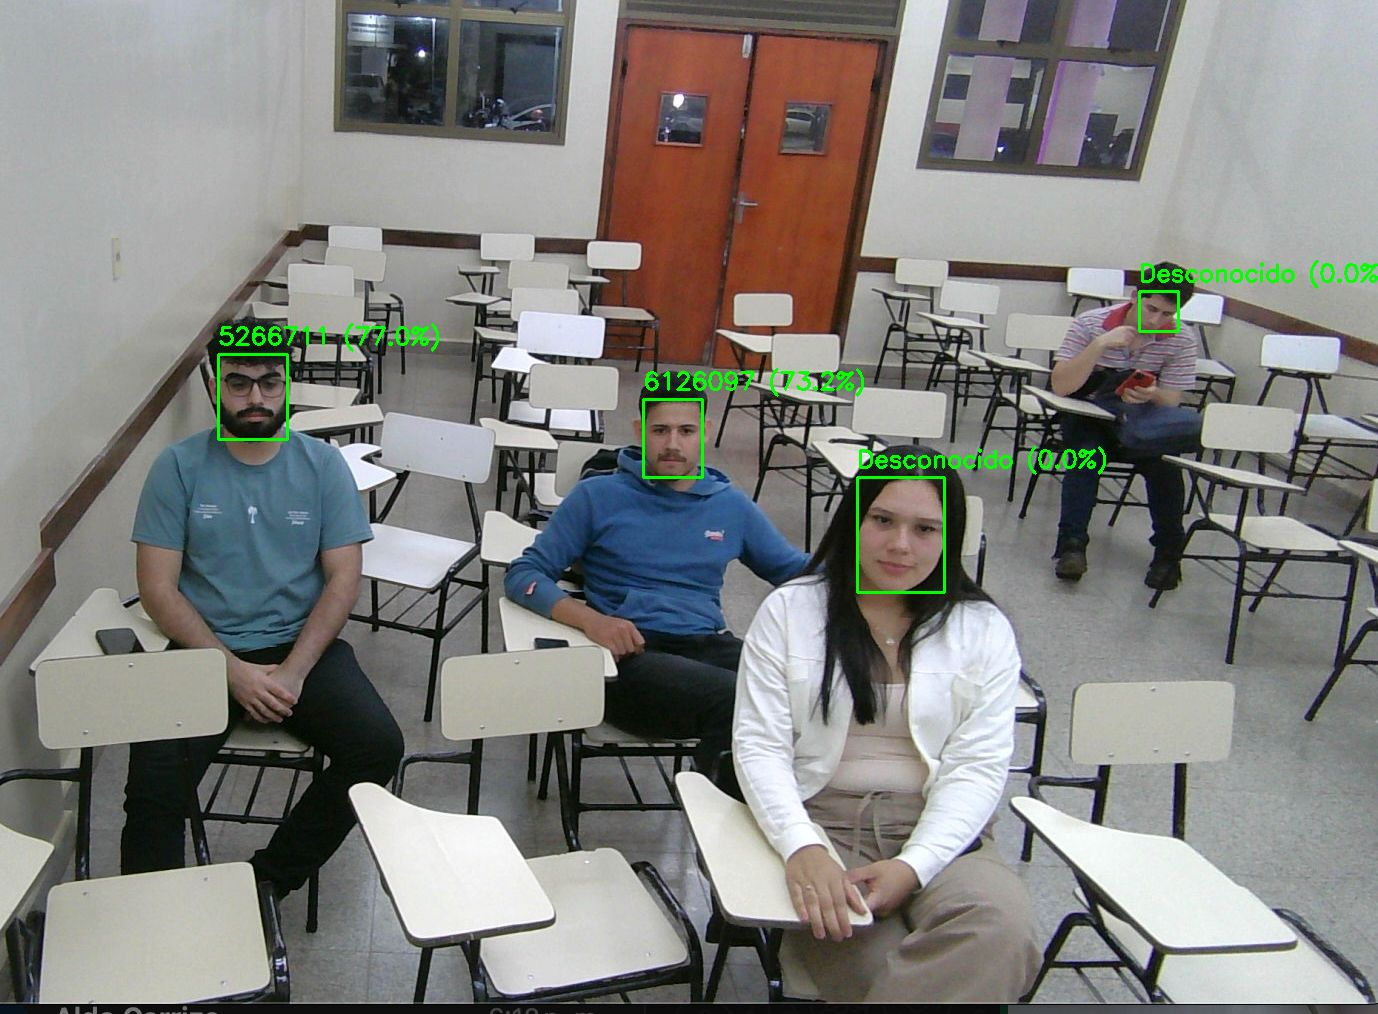
\includegraphics[width=1\textwidth]{capitulo_05/resultados_aula/11.jpg}
    \caption{Prueba con la cámara a una altura de aproximadamente 2,30 metros, mostrando un reconocimiento estable. [Figura Propia]}
    \label{fig:prueba8}
\end{figure}


\textbf{Configuración 9: Prueba con mayor número de participantes registrados}

En la Figura~\ref{fig:prueba9} se observa una prueba con un total de ocho participantes dentro del encuadre, de los cuales seis se encontraban registrados en el sistema. El modelo logró reconocer correctamente a los seis usuarios registrados, alcanzando los niveles de precisión indicados en la tabla de resultados, todos superiores al 80\,\%. La iluminación fue normal durante la captura, permitiendo un desempeño óptimo del modelo ante múltiples detecciones simultáneas en un mismo entorno.

\begin{figure}[H]
    \centering
    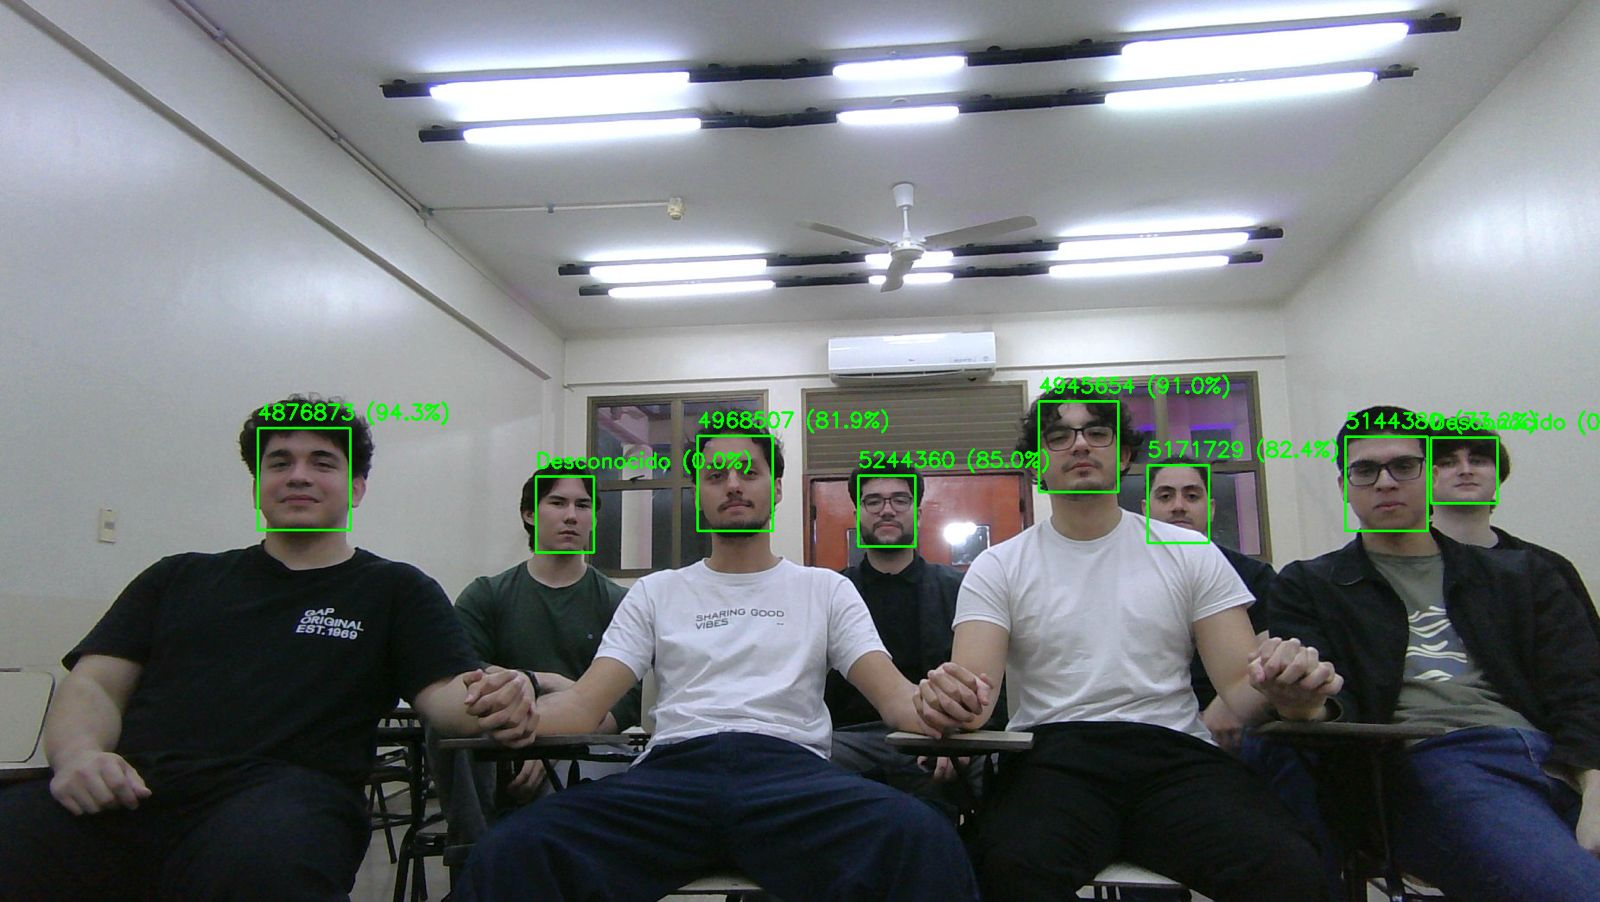
\includegraphics[width=1\textwidth]{capitulo_05/resultados_aula/12.jpg}
    \caption{Prueba con ocho participantes en el encuadre, reconociendo correctamente a los seis usuarios registrados. [Figura Propia]}
    \label{fig:prueba9}
\end{figure}


\textbf{Configuración 10: Prueba grupal con iluminación mínima}

En la Figura~\ref{fig:prueba10} se presenta la misma disposición de participantes de la configuración anterior, pero realizada con la iluminación al mínimo posible dentro del aula. En estas condiciones, el sistema no logró reconocer a ninguno de los usuarios registrados, clasificando todos los rostros como “Desconocido (0.0\,\%)”. Este resultado evidencia la notable dependencia del modelo respecto a una iluminación adecuada, mostrando un descenso total en la precisión cuando la luz ambiental es insuficiente.

\begin{figure}[H]
    \centering
    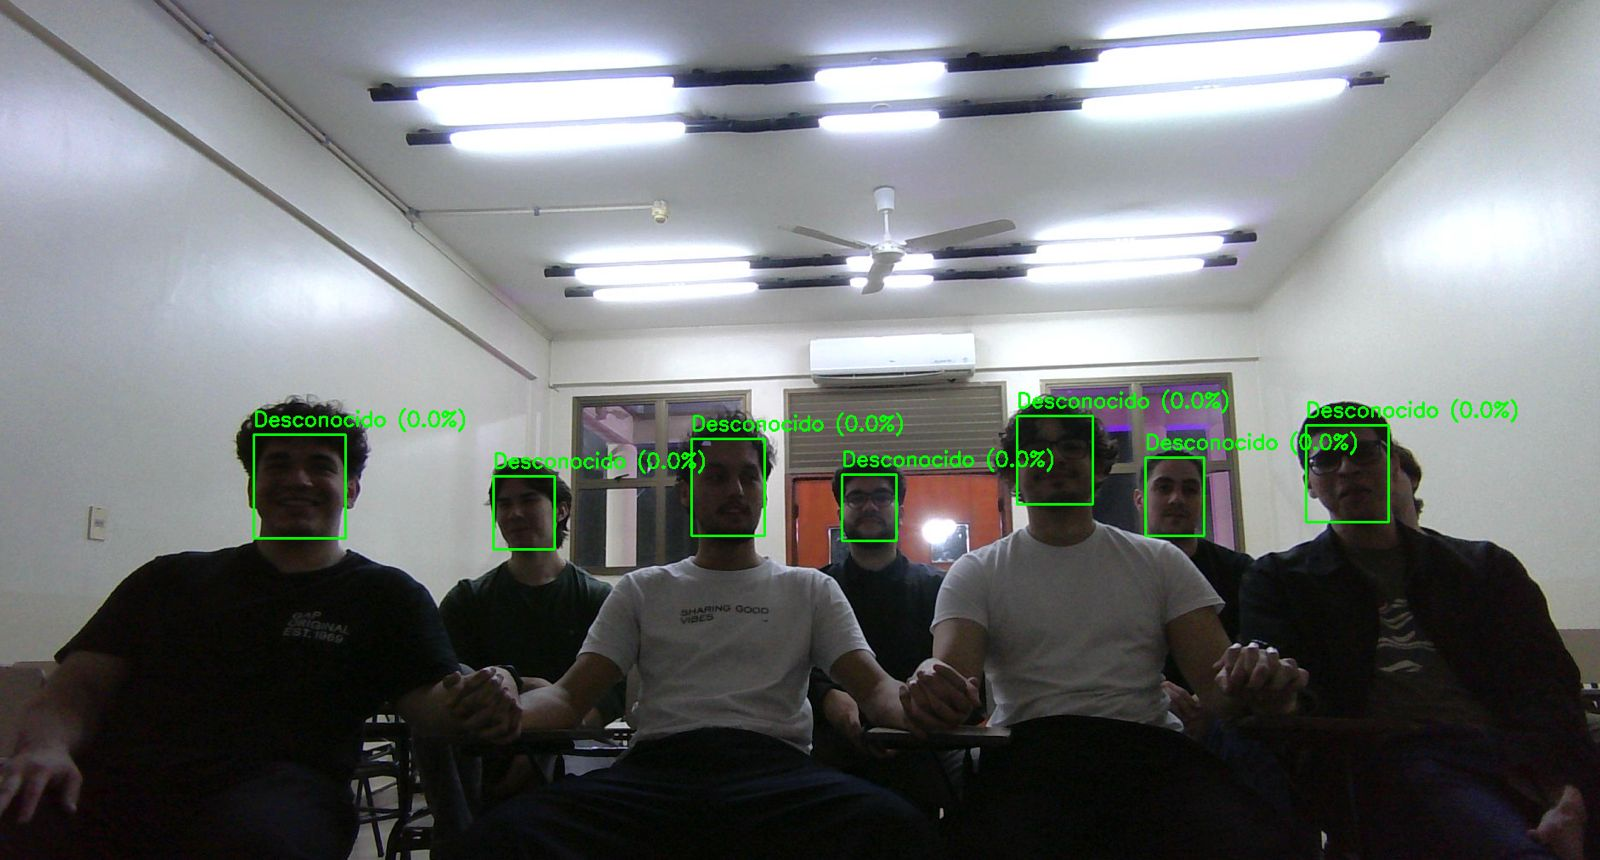
\includegraphics[width=1\textwidth]{capitulo_05/resultados_aula/14.jpg}
    \caption{Prueba grupal con iluminación mínima, sin reconocimiento exitoso de los usuarios registrados. [Figura Propia]}
    \label{fig:prueba10}
\end{figure}

\textbf{Configuración 11: Prueba con variación de distancia y altura de cámara}

En la Figura~\ref{fig:prueba11} se muestra una prueba realizada con la cámara ubicada a una altura aproximada de 2,20 metros respecto a los participantes, bajo condiciones de iluminación ideales. En esta ocasión participaron nueve personas distribuidas de forma heterogénea en el aula, generando distintas distancias y ángulos con relación a la cámara. De los nueve individuos, seis se encontraban registrados en el sistema, y de ellos tres fueron reconocidos correctamente con una similitud superior al 70\,\%. Aunque la distancia y la perspectiva afectaron el reconocimiento de los demás, el sistema logró mantener detecciones estables y un desempeño satisfactorio en condiciones más exigentes, demostrando su capacidad de adaptación ante escenarios con mayor complejidad espacial.

\begin{figure}[H]
    \centering
    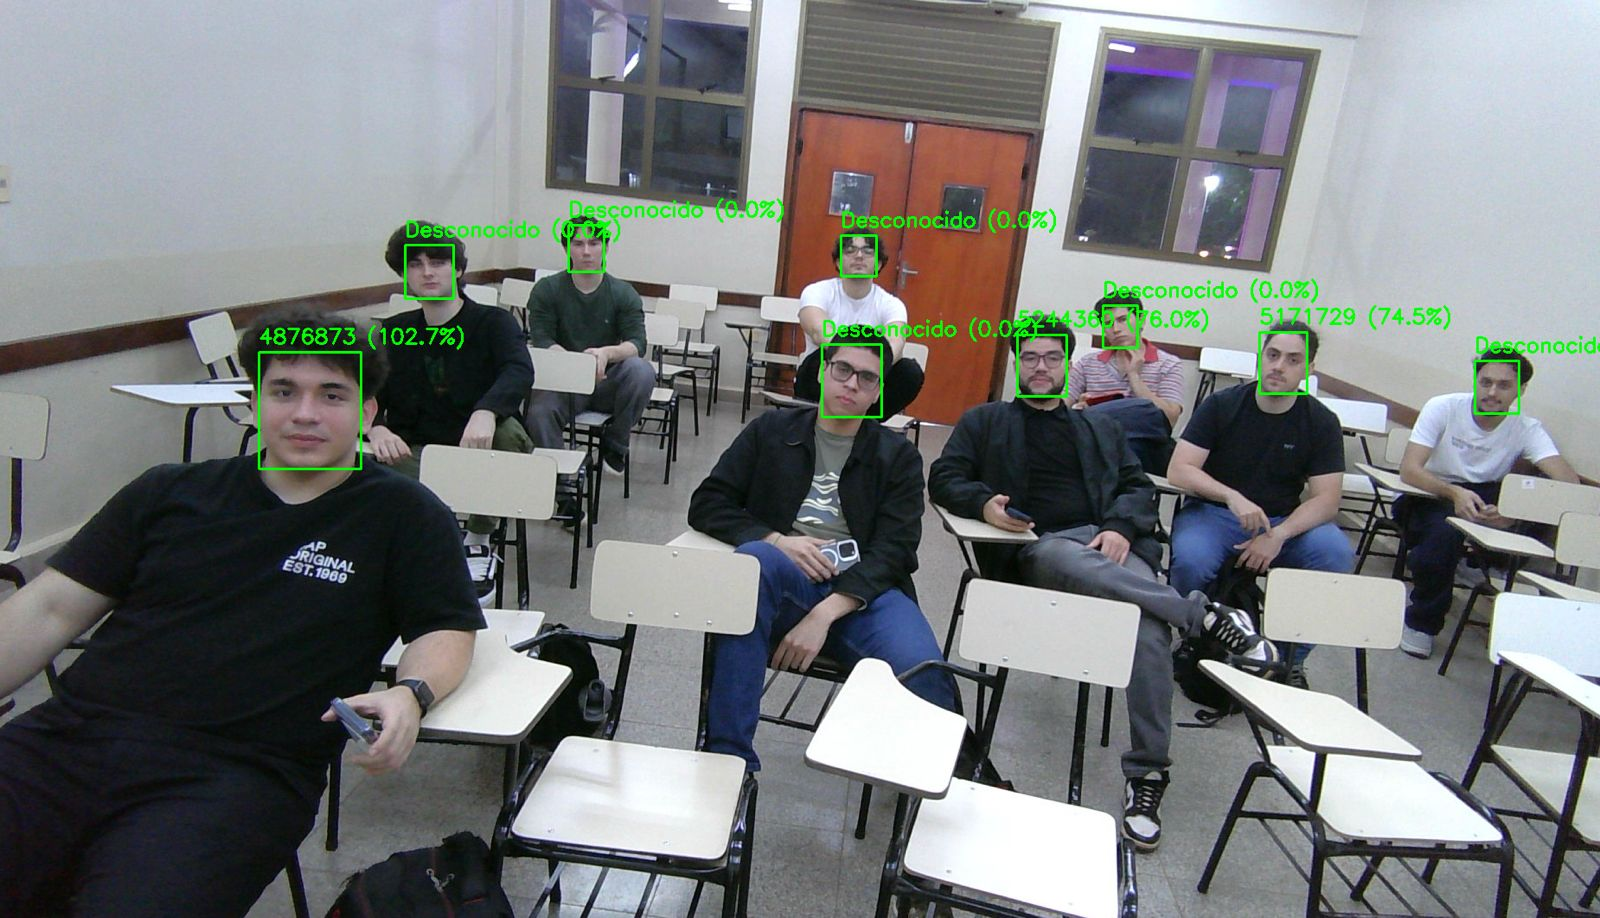
\includegraphics[width=1\textwidth]{capitulo_05/resultados_aula/17.jpg}
    \caption{Prueba con la cámara a 2,20 metros de altura y posiciones diversas de los participantes, evidenciando un desempeño estable. [Figura Propia]}
    \label{fig:prueba11}
\end{figure}

\textbf{Configuración 12: Prueba con variación del ángulo de la cámara}

En la Figura~\ref{fig:prueba12} se presenta la última prueba realizada, en la cual la cámara fue ubicada con un ángulo lateral respecto a los participantes, modificando significativamente la perspectiva habitual utilizada en las capturas anteriores. A pesar de esta variación, el sistema logró mantener una detección estable y reconocer correctamente a los usuarios registrados, conservando niveles de similitud consistentes con las pruebas previas. Estos resultados demuestran que el modelo posee una buena tolerancia ante cambios moderados en el ángulo de visión, manteniendo su rendimiento general dentro de parámetros aceptables.

\begin{figure}[H]
    \centering
    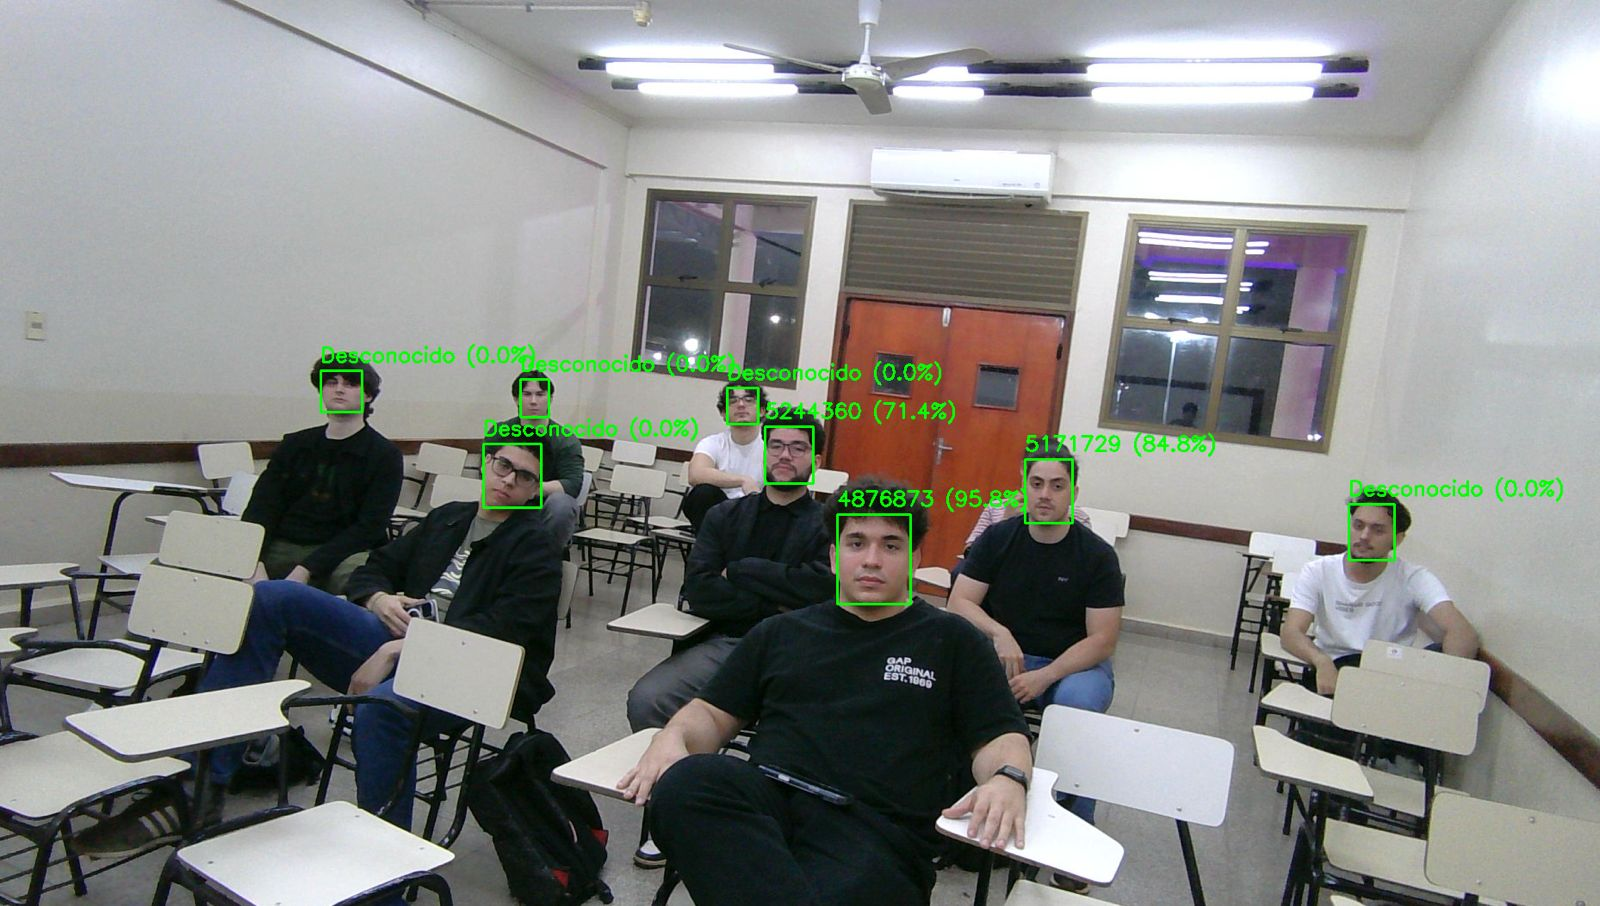
\includegraphics[width=1\textwidth]{capitulo_05/resultados_aula/19.jpg}
    \caption{Prueba final con variación del ángulo de la cámara, mostrando estabilidad en los niveles de similitud. [Figura Propia]}
    \label{fig:prueba12}
\end{figure}



\textbf{Conclusión de las pruebas en aula y análisis de métricas de evaluación}

La Figura~\ref{fig:registrados} muestra la sección de la base de datos correspondiente a los participantes registrados, evidenciando un total de entre 13 y 15 usuarios almacenados con sus respectivos datos de identificación. En la Figura~\ref{fig:entrenamiento} se observa el proceso de procesamiento facial y la generación de vectores de características (\textit{embeddings}) mediante el modelo de reconocimiento. Cada usuario fue representado a partir de múltiples imágenes de entrenamiento, generando centroides únicos empleados durante la fase de verificación facial. Finalmente, la Figura~\ref{fig:asistencias} presenta la tabla de asistencias generada automáticamente, donde se registran las detecciones exitosas y las fechas correspondientes, lo que demuestra el correcto funcionamiento del proceso de identificación y almacenamiento de información.


\begin{figure}[H]
    \centering
    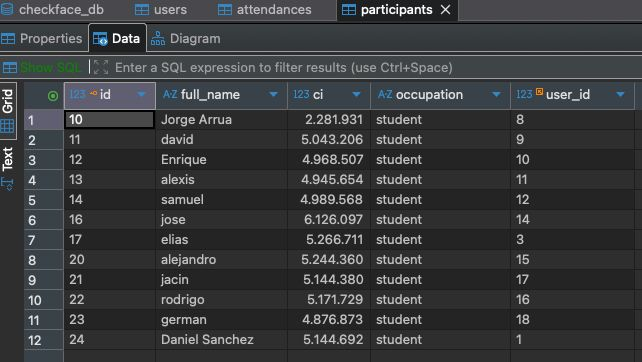
\includegraphics[width=1\textwidth]{capitulo_05/resultados_aula/registrados.jpg}
    \caption{Usuarios registrados dentro del sistema de reconocimiento facial. [Figura Propia]}
    \label{fig:registrados}
\end{figure}

\begin{figure}[H]
    \centering
    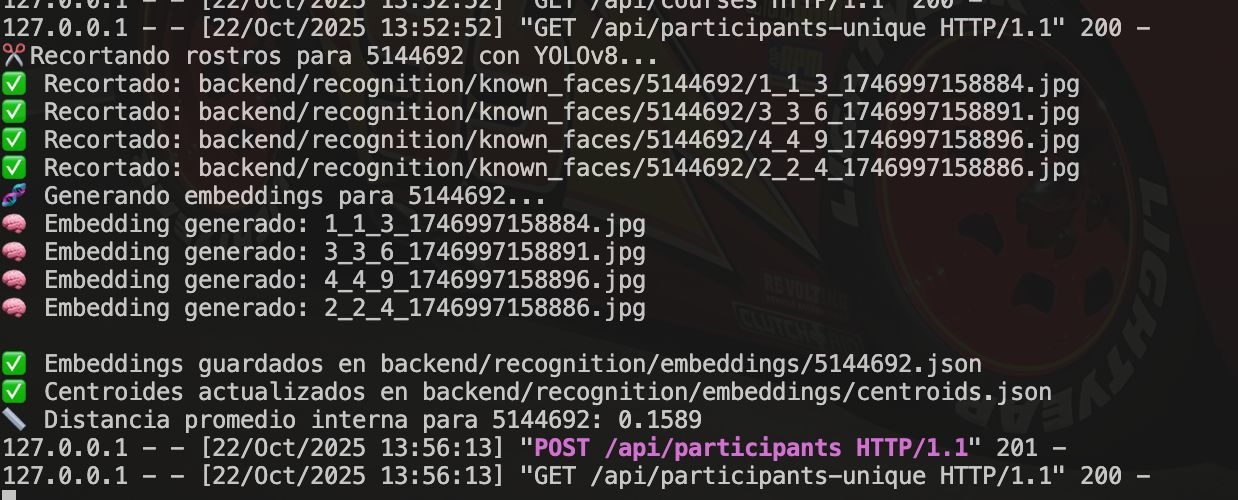
\includegraphics[width=1\textwidth]{capitulo_05/resultados_aula/entrenamiento.jpg}
    \caption{Procesamiento de imágenes y generación de vectores de características (\textit{embeddings}) para cada usuario registrado. [Figura Propia]}
    \label{fig:entrenamiento}
\end{figure}

\begin{figure}[H]
    \centering
    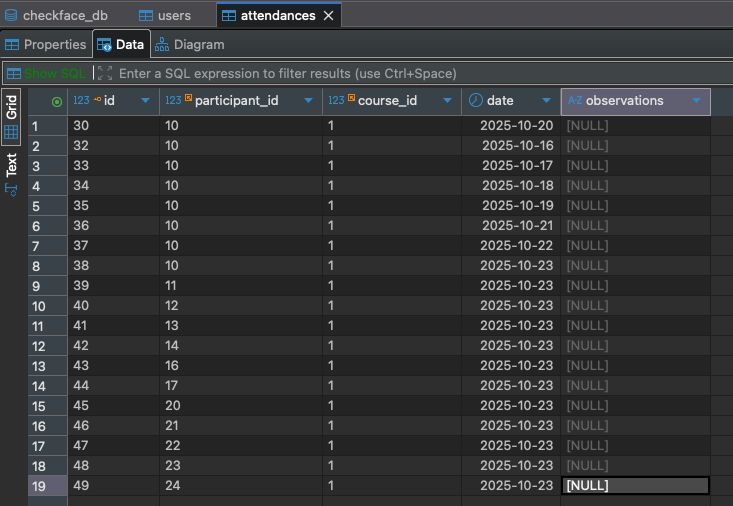
\includegraphics[width=1\textwidth]{capitulo_05/resultados_aula/asistencias.jpg}
    \caption{Registros de asistencias generados automáticamente por el sistema en la base de datos \textit{checkface\_db}. [Figura Propia]}
    \label{fig:asistencias}
\end{figure}



\begin{table}[H]
\centering
\caption{Resumen de métricas obtenidas durante las pruebas finales en aula. [Tabla Propia]}
\label{tab:metricas_finales}
\renewcommand{\arraystretch}{1.3}
\begin{tabular}{|p{3cm}|p{5cm}|p{6cm}|}
\hline
\textbf{Categoría} & \textbf{Métrica} & \textbf{Resultado / Observación} \\ \hline
\multirow{2}{*}{Datos del conjunto} 
& N° de modelos de usuarios & 13–15 modelos registrados con fotografías variadas. \\ \cline{2-3}
& Imágenes por usuario & Mínimo de 5 imágenes por persona para el entrenamiento. \\ \hline

\multirow{3}{*}{Entrenamiento}
& Diversidad visual & Fotografías con variaciones de luz, pose y expresión facial. \\ \cline{2-3}
& Precisión promedio & 80\,\% de detección correcta por fotografía individual. \\ \cline{2-3}
& Pérdida promedio & Error medio controlado, sin sobreajuste evidente. \\ \hline

\multirow{4}{*}{Reconocimiento}
& Umbral configurado & 0.45 (configuración equilibrada entre precisión y tolerancia). \\ \cline{2-3}
& Similitud en condiciones óptimas & Hasta 95\,\%. \\ \cline{2-3}
& Similitud en condiciones complejas & Promedio de 70\,\%. \\ \cline{2-3}
& Tasa de reconocimiento correcto & 90\,\% de usuarios identificados correctamente en aula. \\ \hline

\multirow{2}{*}{Rendimiento }
& Uso promedio de CPU/GPU & Estable, con tiempos de respuesta adecuados. \\ \cline{2-3}
& Tiempo promedio por rostro & Inferior a 300\,ms por detección y verificación. \\ \hline

Validación práctica 
& Tasa de detección real & 8 de cada 10 imágenes correctamente reconocidas. \\ \hline
\end{tabular}
\end{table}
